Prije nego što počnemo govoriti o samom programskom jeziku valjalo bi napomenuti da je Java zapravo i programski jezik i platforma. Neke osnovne informacije o Java programskom jeziku i samoj Java platformi je potrebno znati prije nego što se upustimo u programiranje Java aplikacija.

\section{Programski jezik Java}
Slika~\ref{fig:software-development-process} prikazuje pregled procesa razvoja Java aplikacije.~\cite{javatutorials}

\begin{figure}[h!]
    \label{fig:software-development-process}
    \caption{Proces razvoja Java aplikacije.}
    \centering
    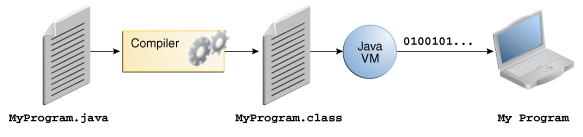
\includegraphics[width=\textwidth]{images/software-development-process}
\end{figure}

U Java programskom jeziku, izvorni kôd (eng. \emph{source code}) je pisan u tekstualnim datotekama. Nazivi tih datoteka završavaju sa .java.

No te datoteke su pisane od strane programera i one, kao takve, nisu razumljive samom procesoru računala kojeg želimo isprogramirati. Taj problem rješava Java prevoditelj (eng. \emph{compiler}) koji će uzeti te datoteke koje su napisane od strane programera i prevesti ih u oblik razumljiv računalu. Dakle, za svaku datoteku koja sadrži izvorni kôd će napraviti po jednu dodatnu datoteku istog naziva samo drugačijeg završetka - \texttt{.class}. Drugim riječima, ako imamo datoteku naziva \texttt{MyProgram.java} tada će prevoditelj proizvesti datoteku naziva \texttt{MyProgram.class}. Postupak prevođenja datoteke koja sadrži izvorni kôd u datoteku koja sadrži Java \emph{bytecode} je opisan sljedećim primjerom: Ako postoji izvorni kôd napisan u \texttt{MyProgram.java} datoteci koju želimo prevesti u \texttt{MyProgram.class} datoteku koja sadrži Java \emph{bytecode} onda moramo u naredbenom retku upisati sljedeće:

\begin{lstlisting}
    $ javac MyProgram.java
\end{lstlisting}

Nakon toga, pritiskom na tipku \texttt{Enter} će se pozvati Java prevoditelj, \texttt{javac}\footnote{\label{ftn:javaandjavac}\texttt{javac} i \texttt{java} su alati implementirani od strane Oracle Corporation. Oni su samo neki od alata koji se nalaze u JDK (\emph{Java Development Kit}) i JRE (\emph{Java Runtime Environment}) koji su dostupani za besplatno preuzimanje sa \url{http://www.oracle.com/technetwork/java/}.}, koji će onda prevesti \texttt{MyProgram.java} u Java \emph{bytecode}.

Kao što je i rečeno, \texttt{.class} datoteke sadrže podatke koje su razumljive isključivo računalu za razliku od izvornog kôda koji je razumljiv isključivo programeru.

\begin{infobox}
    Nazivi datoteka koje sadržavaju izvorni kôd pisan u Java jeziku moraju završavati sa \texttt{.java}.
\end{infobox}

No tu priča zapravo ne prestaje. Ranije je rečeno da su datoteke koje Java prevoditelj stvara razumljive računalu, no to nije sasvim istina. \texttt{.class} datoteke zapravo ne sadrže kôd kojeg procesor vašeg računala može razumjeti i izvršavati. Umjesto toga \texttt{.class} datoteke sadrže \emph{bytecode} - jezik Java virtualne mašine (JVM).

\begin{infobox}
    Java aplikacija se sastoji od više \texttt{.class} datoteka grupiranih u direktorije.
\end{infobox}

JVM je ta komponenta koja zna čitati \texttt{.class} datoteke i izvršavati njih. Tj. JVM se pokreće kada se želi izvršavati aplikacija pisana u Java programskom jeziku, čita \texttt{.class} datoteke koje čine tu aplikaciju te iz njih zapravo stvara strojni kôd (eng. \emph{native code}) pomoću kojeg se onda upravlja procesorom.

Da bi pokrenuli ranije prevođenu datoteku \texttt{MyProgram.class} pomoću JVM, moramo koristiti sljedeću naredbu u naredbenom retku:

\begin{lstlisting}
    $ java MyProgram
\end{lstlisting}

java\footnote{Više o \texttt{java} alatu možete pročitati na fusnoti \ref{ftn:javaandjavac}.} je alat pomoću kojega možemo pokretati aplikacije pisane u Java programskom jeziku.

\section{Java virtualna mašina}
Java virtualna mašina je ključna komponenta cijele Java platforme te vrijedi spomenuti par činjenica tako da se dobije bolja predodžba i da se poveća razumijevanje cjelokupne Java tehnologije. S tim rečeno, promotrimo sliku~\ref{fig:java-platform-benefits}~\cite{javatutorials}.

\begin{figure}[h!]
    \label{fig:java-platform-benefits}
    \caption{Prednosti Java platforme.}
    \centering
    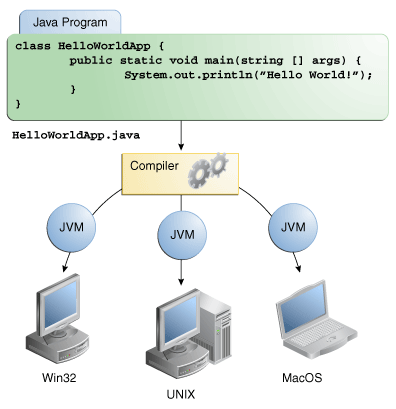
\includegraphics[scale=0.6]{images/java-platform-benefits.png}
\end{figure}

Slika zapravo prikazuje najveću prednost Java tehnologije nad drugim rješenjima. "Write once, run anywhere"~\cite{writeoncerunanywhere} je Sun Microsystem slogan koji ilustrira \emph{cross-platform} mogućnosti Java platforme.

Ono što je tvrtka Sun Microsystem zamislila je to da programer piše jedan jedinstveni izvorni kôd koji se prevodi te se kao takav može izvršavati na bilo kojoj Java virtualnoj mašini. Drugim riječima, vaša aplikacija se može izvršavati na Microsoft Windows, GNU/Linux, Mac OS operacijskim sustavima bez bilo kakvog prethodnog dodatnog prilagođavanja i promjene izvornog kôda.

Ono što je isto tako bitno naglasiti je to da se izvorni kôd može prevesti na bilo kojoj platformi na kojoj je sama Java platforma instalirana.

Zašto je to bitno, tj. koje su tu prednosti u odnosu na druga rješenja?

\begin{itemize}
    \item Programeri održavaju samo jedan \emph{codebase}\footnote{Termin codebase predstavlja jednu cijelu kolekciju izvornog kôda koji sačinjava aplikaciju. Kada se kaže da neka aplikacija ili projekt ima \emph{multiple codebases} ili više kolekcija izvornog kôda to znači da je svaka kolekcija jedna nezavisna implementacija te aplikacije ili projekta. Primjerice, planetarno popularna aplikacija \emph{Skype} zapravo ima više nezavisnih implementacija - Android, Windows Phone, iPhone itd.}. To znači da je puno manji broj grešaka u aplikaciji, te da se greške lakše ispravljaju.
    
    \item Prevođenje izvornog kôda za konkretnu platformu i cross-compiling\footnote{\emph{Cross-compiling} je proces koji omogućava da prevodite izvorni kôd za platformu različitu od one na kojem je taj prevoditelj instaliran. Primjerice, \emph{cross compiler} je potreban za prevođenje izvornog kôda za nekakav ugrađeni sustav (eng. \emph{embedded system}) ili mikrokontroler zato što takvi uređaji nemaju operacijski sustav.} uopće više nije ni potreban. Dakle, prevodite izvorni kôd na bilo kojoj platformi da bi se izvršavao na bilo kojoj platformi. To znači da je distribucija vaše aplikacije puno brža u odnosu na druga riješenja.
    
    \item Kupac, klijent ili korisnik vaše aplikacije može mijenjati arhitekturu i/ili operacijski sustav na kojem će se izvršavati aplikacija. Drugim riječima, ako je vaš \emph{codebase} vezan za arhitekturu ili operacijski sustav onda vi morate i prilagoditi vaš izvorni kôd da bi ste podržavali neku drugu, dodatnu arhitekturu ili operacijski sustav. Naravno da takav zahvat traži dodatno vrijeme i znanje i dodatne potencijalne probleme. Java tehnologija vas izolira od takvih problema.
\end{itemize}

\section{Java platforma}